\subsection{概述}
\label{subsec:sgxdedup-arch}

图~\ref{fig:sgxdedup-overview}展示了\sysnameS 的系统框架,其分别在密钥服务器和每个客户端中引入了密钥安全区\textit{(Key Enclave)}和所有权证明安全区\textit{(PoW Enclave)}。

\begin{figure}[!htb]
    \centering
    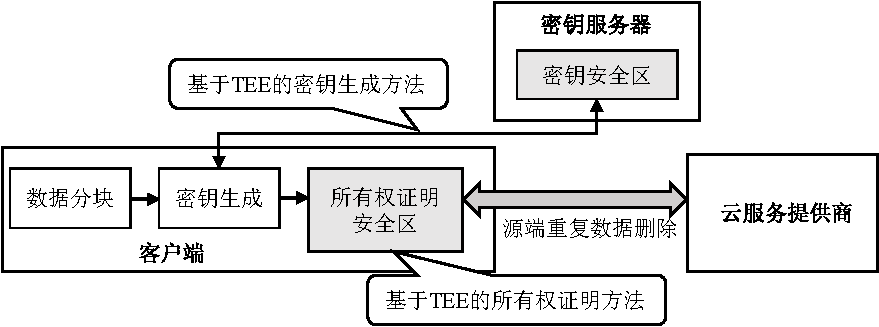
\includegraphics[width=0.9\textwidth]{pic/sgxdedup/sgxdedup-arch.pdf}
    \caption{\sysnameS 系统框架,在密钥服务器和每个客户端中分别部署了密钥安全区和所有权证明安全区}
    \label{fig:sgxdedup-overview}
\end{figure}

\paragraph*{基于密钥安全区的服务器MLE密钥生成。}如图~\ref{fig:sgxdedup-overview-key}所示,\sysnameS 在密钥服务器中部署一个密钥安全区\textit{(Key Enclave)},以管理和保护服务器辅助消息锁加密所需的的全局秘密$S$,使其免受恶意(例如,被攻击者攻击并取得控制权限)的密钥服务器的威胁。在执行服务器辅助消息锁加密密钥生成时,密钥安全区和客户端都首先基于共享的会话密钥(Blinded key)建立一个安全信道(有关如何生成会话密钥的详细设计,请参阅\S\ref{subsec:sgxdedup-key-management});然后客户端通过安全信道提交明文数据块的指纹;密钥安全区计算全局秘密和数据块指纹连接的结果的安全哈希作为该指纹对应的消息锁加密密钥;最后,密钥安全区通过安全信道向客户端返回该消息锁加密密钥。

\begin{figure}[!htb]
    \centering
    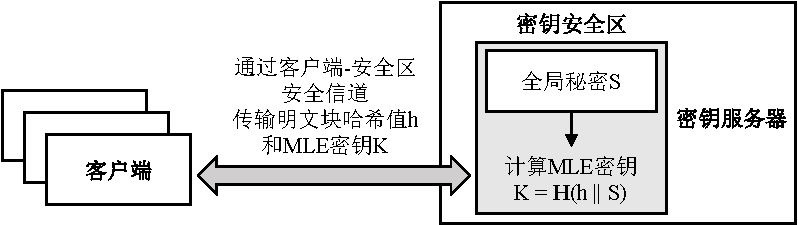
\includegraphics[width=0.8\textwidth]{pic/sgxdedup/key-enclave.pdf}
    \caption{基于密钥安全区的服务器辅助MLE密钥生成}
    \label{fig:sgxdedup-overview-key}
\end{figure}

密钥安全区同时实现了性能和安全性目标,它避免了在消息锁加密密钥生成期间使用昂贵的OPRF协议\cite{bellare2013DupLESS}。此外,它通过基于共享的会话密钥的安全信道保护数据块指纹和消息锁加密密钥,这样密钥服务器就无法从消息锁加密密钥生成过程中学习任何信息。此外,它可以有效保护安全区内存中的全局秘密$S$,即使密钥服务器受到攻击也能避免全局秘密的泄露,保障服务器辅助消息锁加密的安全性。但传统服务器辅助消息锁加密的安全性会由于全局秘密泄露而降低(\S\ref{subsec:background-encrypted-deduplication-key})。



\paragraph*{基于所有权证明安全区的数据块所有权证明。}如图~\ref{fig:sgxdedup-overview-pow}所示,\sysnameS 在每个客户端中部署一个所有权证明安全区,以证明源端重复数据删除中密文数据块的真实性。所有权证明安全区首先与云服务端协商生成一个共享的所有权PoW密钥\textit{PoW}密钥(本文目前使用Diffie-Hellman密钥交换(DHKE)实现密钥协商,参见\S\ref{sec:sgxdedup-implementation})。在生成消息锁加密密钥后,客户端将每个明文数据块加密为密文数据块。所有权证明安全区将密文数据块作为输入,计算相应的指纹,并使用与云服务端共享的PoW密钥创建该指纹的签名。随后,客户端将指纹和签名一起上传到云服务端。云服务端根据客户端对应PoW密钥及指纹附加的签名验证指纹的真实性。只有当指纹被认证为真实有效时,云服务端才会继续检查指纹是否对应于任何已经存储的密文数据块副本。这里,本文验证客户端对密文数据块的所有权而不是明文的所有权(例如,\cite{halevi11}),以保护原始信息不被云服务端访问。由于消息锁加密产生的密文数据块与明文数据块一一对应,并且密文数据块的所有权与对应的明文数据块的所有权一致。因此,确保密文数据块的所有权足以保证安全。

\begin{figure}[!htb]
    \centering
    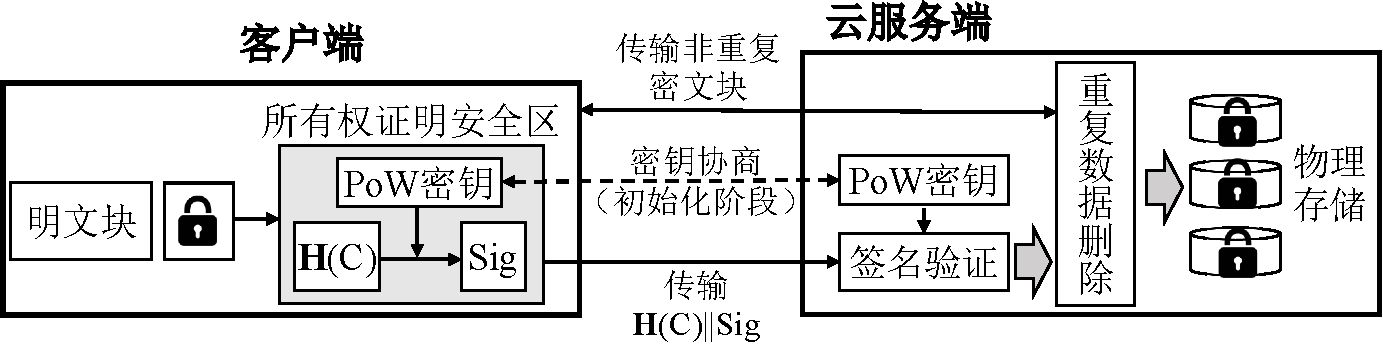
\includegraphics[width=\textwidth]{pic/sgxdedup/pow.pdf}
    \caption{\sysnameS 系统架构: 所有权证明安全区}
    \label{fig:sgxdedup-overview-pow}
\end{figure}


与密钥安全区相似,所有权证明安全区同样可实现效率与安全性的双重设计目标。它避免了基于密码学算法的所有权证明中Merkle树等结构的计算开销。同时,由于数据块是否已被云服务端存储的信息仅在数据块所有权验证通过后才会返回客户端,密钥安全区可有效保护重复数据删除系统免受恶意客户端的造数据所有权的攻击威胁。

\textbf{与现有研究\cite{kim2019ShieldStore,fuhry2020segshare,djoko2019NEXUS}在安全区内执行密钥生成和加密不同,本文选择在安全区之外执行数据块加密。}主要原因是原始明文数据块和加密过程都位于客户端内。被攻击的客户端本身可以直接访问其明文数据块,将加密过程移动到安全区内并不能提高安全性,同时还会导致安全区的计算开销增大、可信计算基大小增加。

\begin{table}[!htb]
    \small
    \centering
    \begin{tabular}{ccc}
        \toprule
        {\bf 所属安全区} & {\bf ECall名称}            & {\bf 描述}                                                           \\ 
        \midrule
        \multirow{5}{*}{\bf 密钥安全区}
                         & \textit{Secret generation} & 产生全局秘密 
        (\S\ref{subsec:sgxdedup-enclave-management})                                                                         \\
                         & \textit{Rekeying}          & 更新会话密钥 
        (\S\ref{subsec:sgxdedup-key-management})                                                                             \\
                         & \textit{Nonce checking}    & 检查nonce合规性 
        (\S\ref{subsec:sgxdedup-encryption})                                                                                 \\
                         & \textit{Key generation}    & 产生消息锁加密(MLE)密钥 (\S\ref{subsec:sgxdedup-encryption})         \\
                         & \textit{Mask generation}   & 生成加密掩码 (\S\ref{subsec:sgxdedup-encryption})                    \\
        \hline
        \multirow{3}{*}{\bf 所有权证明安全区}
                         & \textit{Key unsealing}     & 从磁盘解封所有权PoW密钥 (\S\ref{subsec:sgxdedup-enclave-management}) \\
                         & \textit{Key sealing}       & 密封所有权PoW密钥至磁盘 (\S\ref{subsec:sgxdedup-enclave-management}) \\
                         & \textit{Proof generation}  & 签名密文数据块对应的指纹 
        (\S\ref{sec:sgxdedup-implementation})                                                                                \\
        \bottomrule
    \end{tabular}
    \caption{\sysnameS 中的安全区内部调用(Ecalls)}
    \label{tab:sgxdedup-ecall}
\end{table}

\paragraph*{部署安全区存在的问题。}有效地​​实现基于TEE的加密后重复数据删除并非易事,因为本文需要减轻安全区的潜在性能开销,否则会抵消引入安全区带来的整体性能优势。本文提出了以下三个关键科学问题,并基于一套用于密钥安全区和所有全证明安全区(Table~\ref{tab:sgxdedup-ecall})的安全区内部调用来解决这些问题。

\begin{itemize}[leftmargin=0em]
    \item \textbf{如何安全有效地引导安全区?} (\S\ref{subsec:sgxdedup-enclave-management})由于密钥安全区需要维护全局秘密,在安全区启动时将全局秘密安全地载入密钥安全区中至关重要。此外,所有权证明安全区与客户端深度绑定,它应该在客户端在线访问云服务端时快速且安全的启动,并在客户端退出时以安全有效的方式终止。
    \item \textbf{密钥安全区和每个客户端应该如何建立安全信道?} (\S\ref{subsec:sgxdedup-key-management})
          每个客户端都基于共享的会话密钥与密钥安全区进行安全通信,以便生成必要的消息锁加密密钥来保护外包数据块。由于客户端可能随时加入或退出云存储服务订阅组,会话密钥不仅需要被高效协商产生,而且需要可以动态更新以进行动态客户端认证。
    \item \textbf{密钥安全区应该如何减少管理客户端安全信道的计算开销?} (\S\ref{subsec:sgxdedup-encryption})
          在每个安全信道中(密钥安全区和每个客户端之间),密钥安全区需要解密收到的数据块指纹并加密所生成的消息锁加密密钥。它的计算复杂度随着指纹数量和连接客户端的数量增加而增加。
\end{itemize}
